% begin module volumes-ex-two-curves
\begin{frame}
\begin{example}[Example]
Find the volume of the solid obtained by rotating about the line $y = 1$ the region between $y = \sqrt{x}$ and $y = x^2$.
\begin{columns}[c]
\column{.4\textwidth}
%\begin{center}
%\only<1>{%
%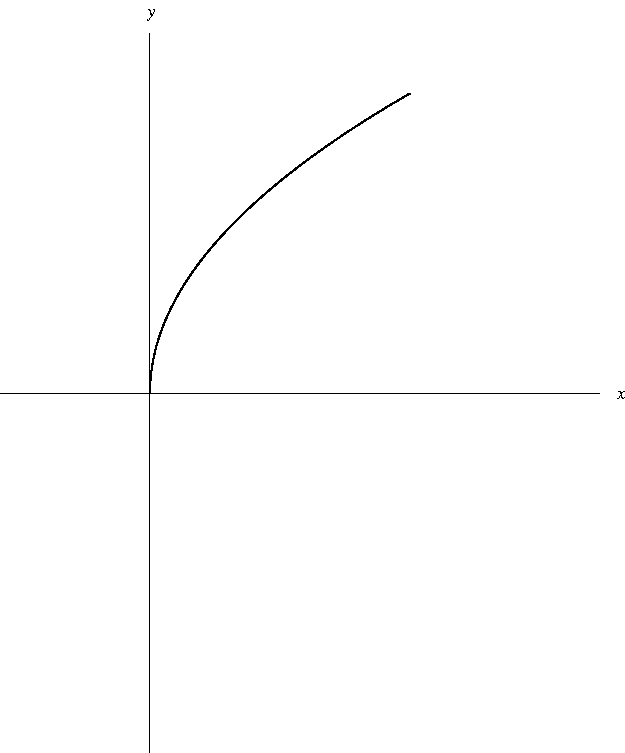
\includegraphics[height=3.5cm]{TESTING/pictures/06-02-ex2a.pdf} %
%}%
%\only<2>{%
%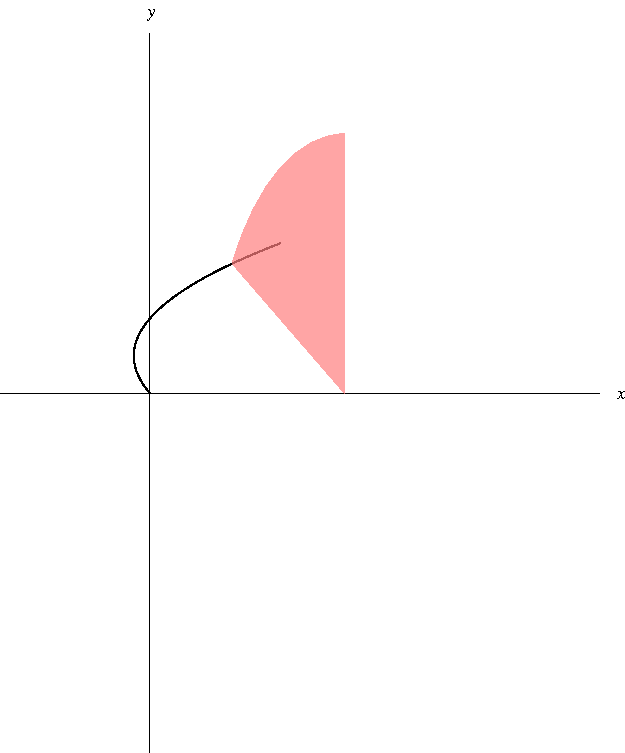
\includegraphics[height=3.5cm]{TESTING/pictures/06-02-ex2b.pdf} %
%}%
%\only<3>{%
%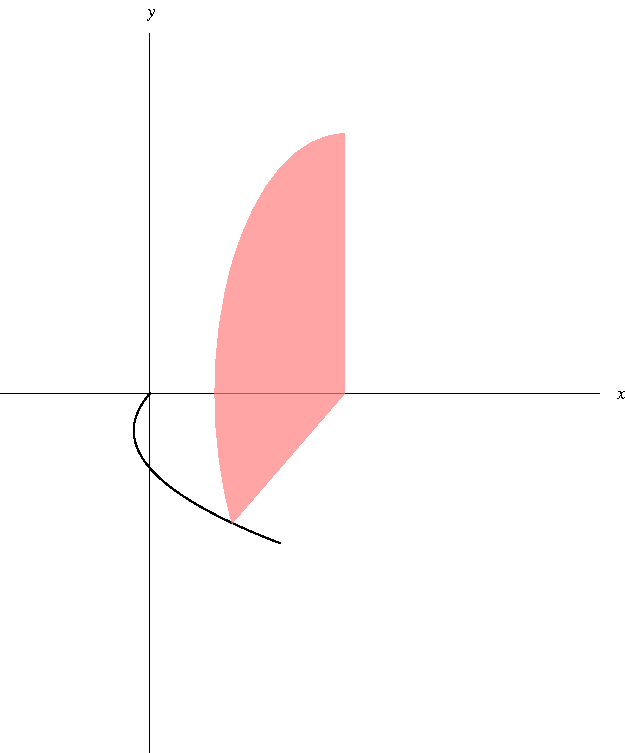
\includegraphics[height=3.5cm]{TESTING/pictures/06-02-ex2c.pdf} %
%}%
%\only<4>{%
%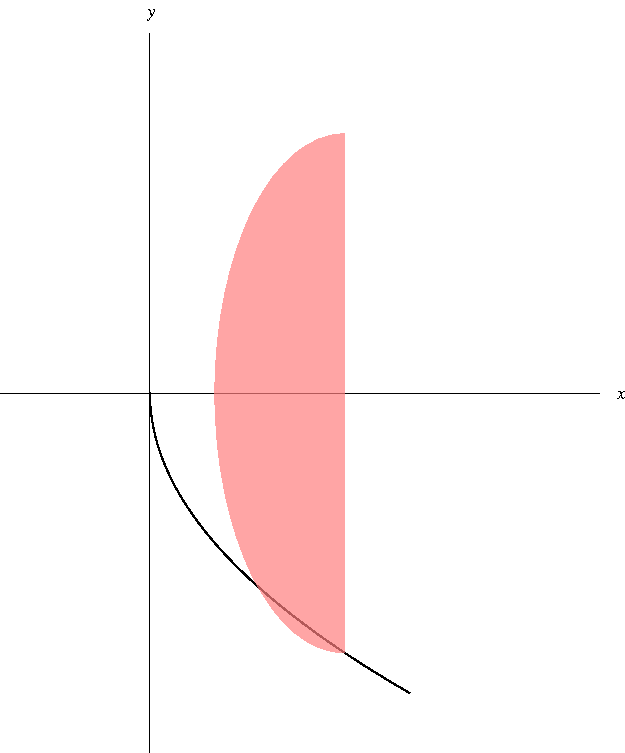
\includegraphics[height=3.5cm]{TESTING/pictures/06-02-ex2d.pdf} %
%}%
%\only<5>{%
%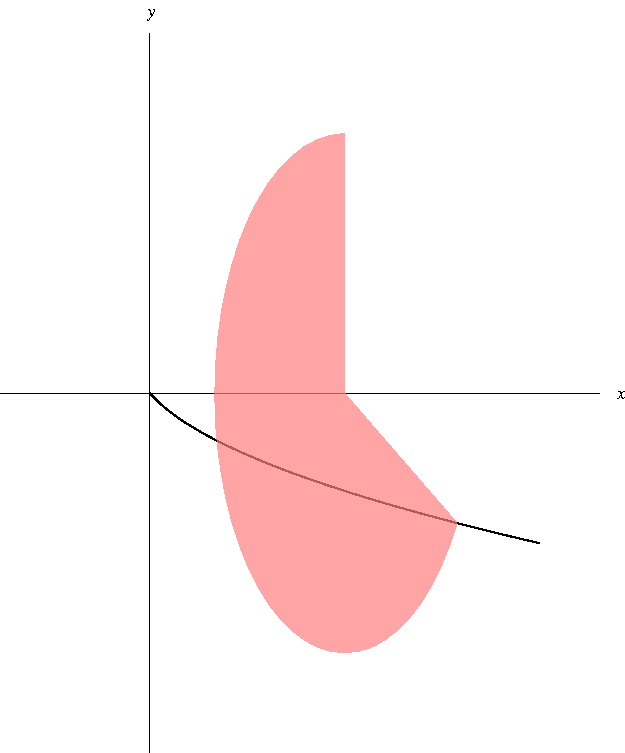
\includegraphics[height=3.5cm]{TESTING/pictures/06-02-ex2e.pdf} %
%}%
%\only<6>{%
%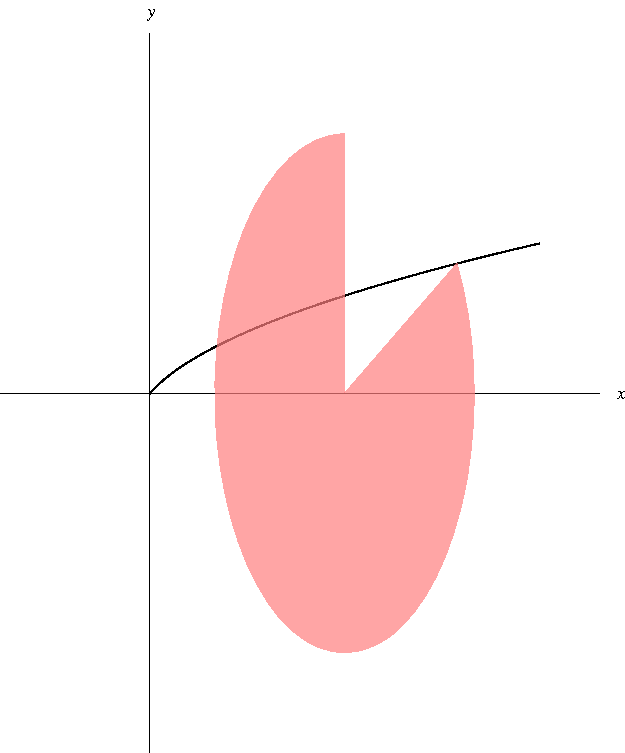
\includegraphics[height=3.5cm]{TESTING/pictures/06-02-ex2f.pdf} %
%}%
%\only<7->{%
%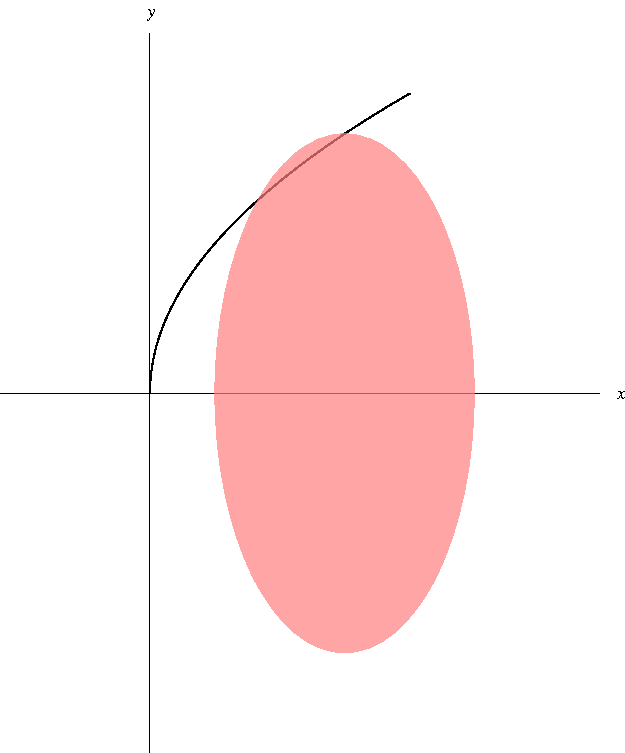
\includegraphics[height=3.5cm]{TESTING/pictures/06-02-ex2g.pdf} %
%}%
%\end{center}
empty for now
\column{.6\textwidth}
\begin{itemize}
\item<1->  Points of intersection: $0$ and $1$.
\item<1->  The cross-section through the point $(x, 0)$ is washer-shaped.
\item<1->  Inner radius: $1 - \sqrt{x}$.  Outer radius: $1 - x^2$.
\item<1->  The area of across-section is $A(x) = \left( \pi x (1-\sqrt{x})^2 - \pi (1-x^2)^2\right)$.
\end{itemize}
\end{columns}
\abovedisplayskip=0pt
\belowdisplayskip=0pt
\begin{eqnarray*}
\uncover<1->{%
V%
}%
 & \uncover<1->{ = } &  %
\uncover<1->{%
\int_0^1 \pi \left( (1-\sqrt{x})^2 - (1 - x^2)^2\right) \ \diff x%
}%
 \uncover<1->{ = }  %
\uncover<1->{%
\int_0^1 \pi \left( (1-2x +x^4) - (1-2x^4+x^8)\right) \ \diff x%
}\\%
& \uncover<1->{ = } & %
\uncover<1->{%
\int_0^1 \pi \left( x^8 + 3x^4 - 2x \right) \ \diff x%
}%
 \uncover<1->{ = } %
\uncover<1->{%
\pi \left[ 4x^2 - x^3 - x^4 + \frac{1}{5}x^5 \right]_0^1%
}%
 \uncover<1->{ = } %
\uncover<1->{%
\frac{\pi}{2}%
}%
\end{eqnarray*}
\end{example}
\end{frame}
% end module volumes-ex-two-curves
